\documentclass[tikz,border=6pt]{standalone}
\usetikzlibrary{calc}

% Gerado pelo MOIRA a partir do diagrama.
%
% Documento completo: compila direto com pdflatex.
%
% As posições são coordenadas nomeadas: mover um tensor é mudar uma linha
% da lista abaixo, e as pernas e as curvas o acompanham.

% Paleta da identidade MOIRA. Trocar a figura inteira de cor é mudar aqui.
\definecolor{moiraInk}{HTML}{1B2430}
\definecolor{moiraGreen}{HTML}{228833}
\definecolor{moiraAmber}{HTML}{CCBB44}
\definecolor{moiraPurple}{HTML}{AA3377}

\begin{document}
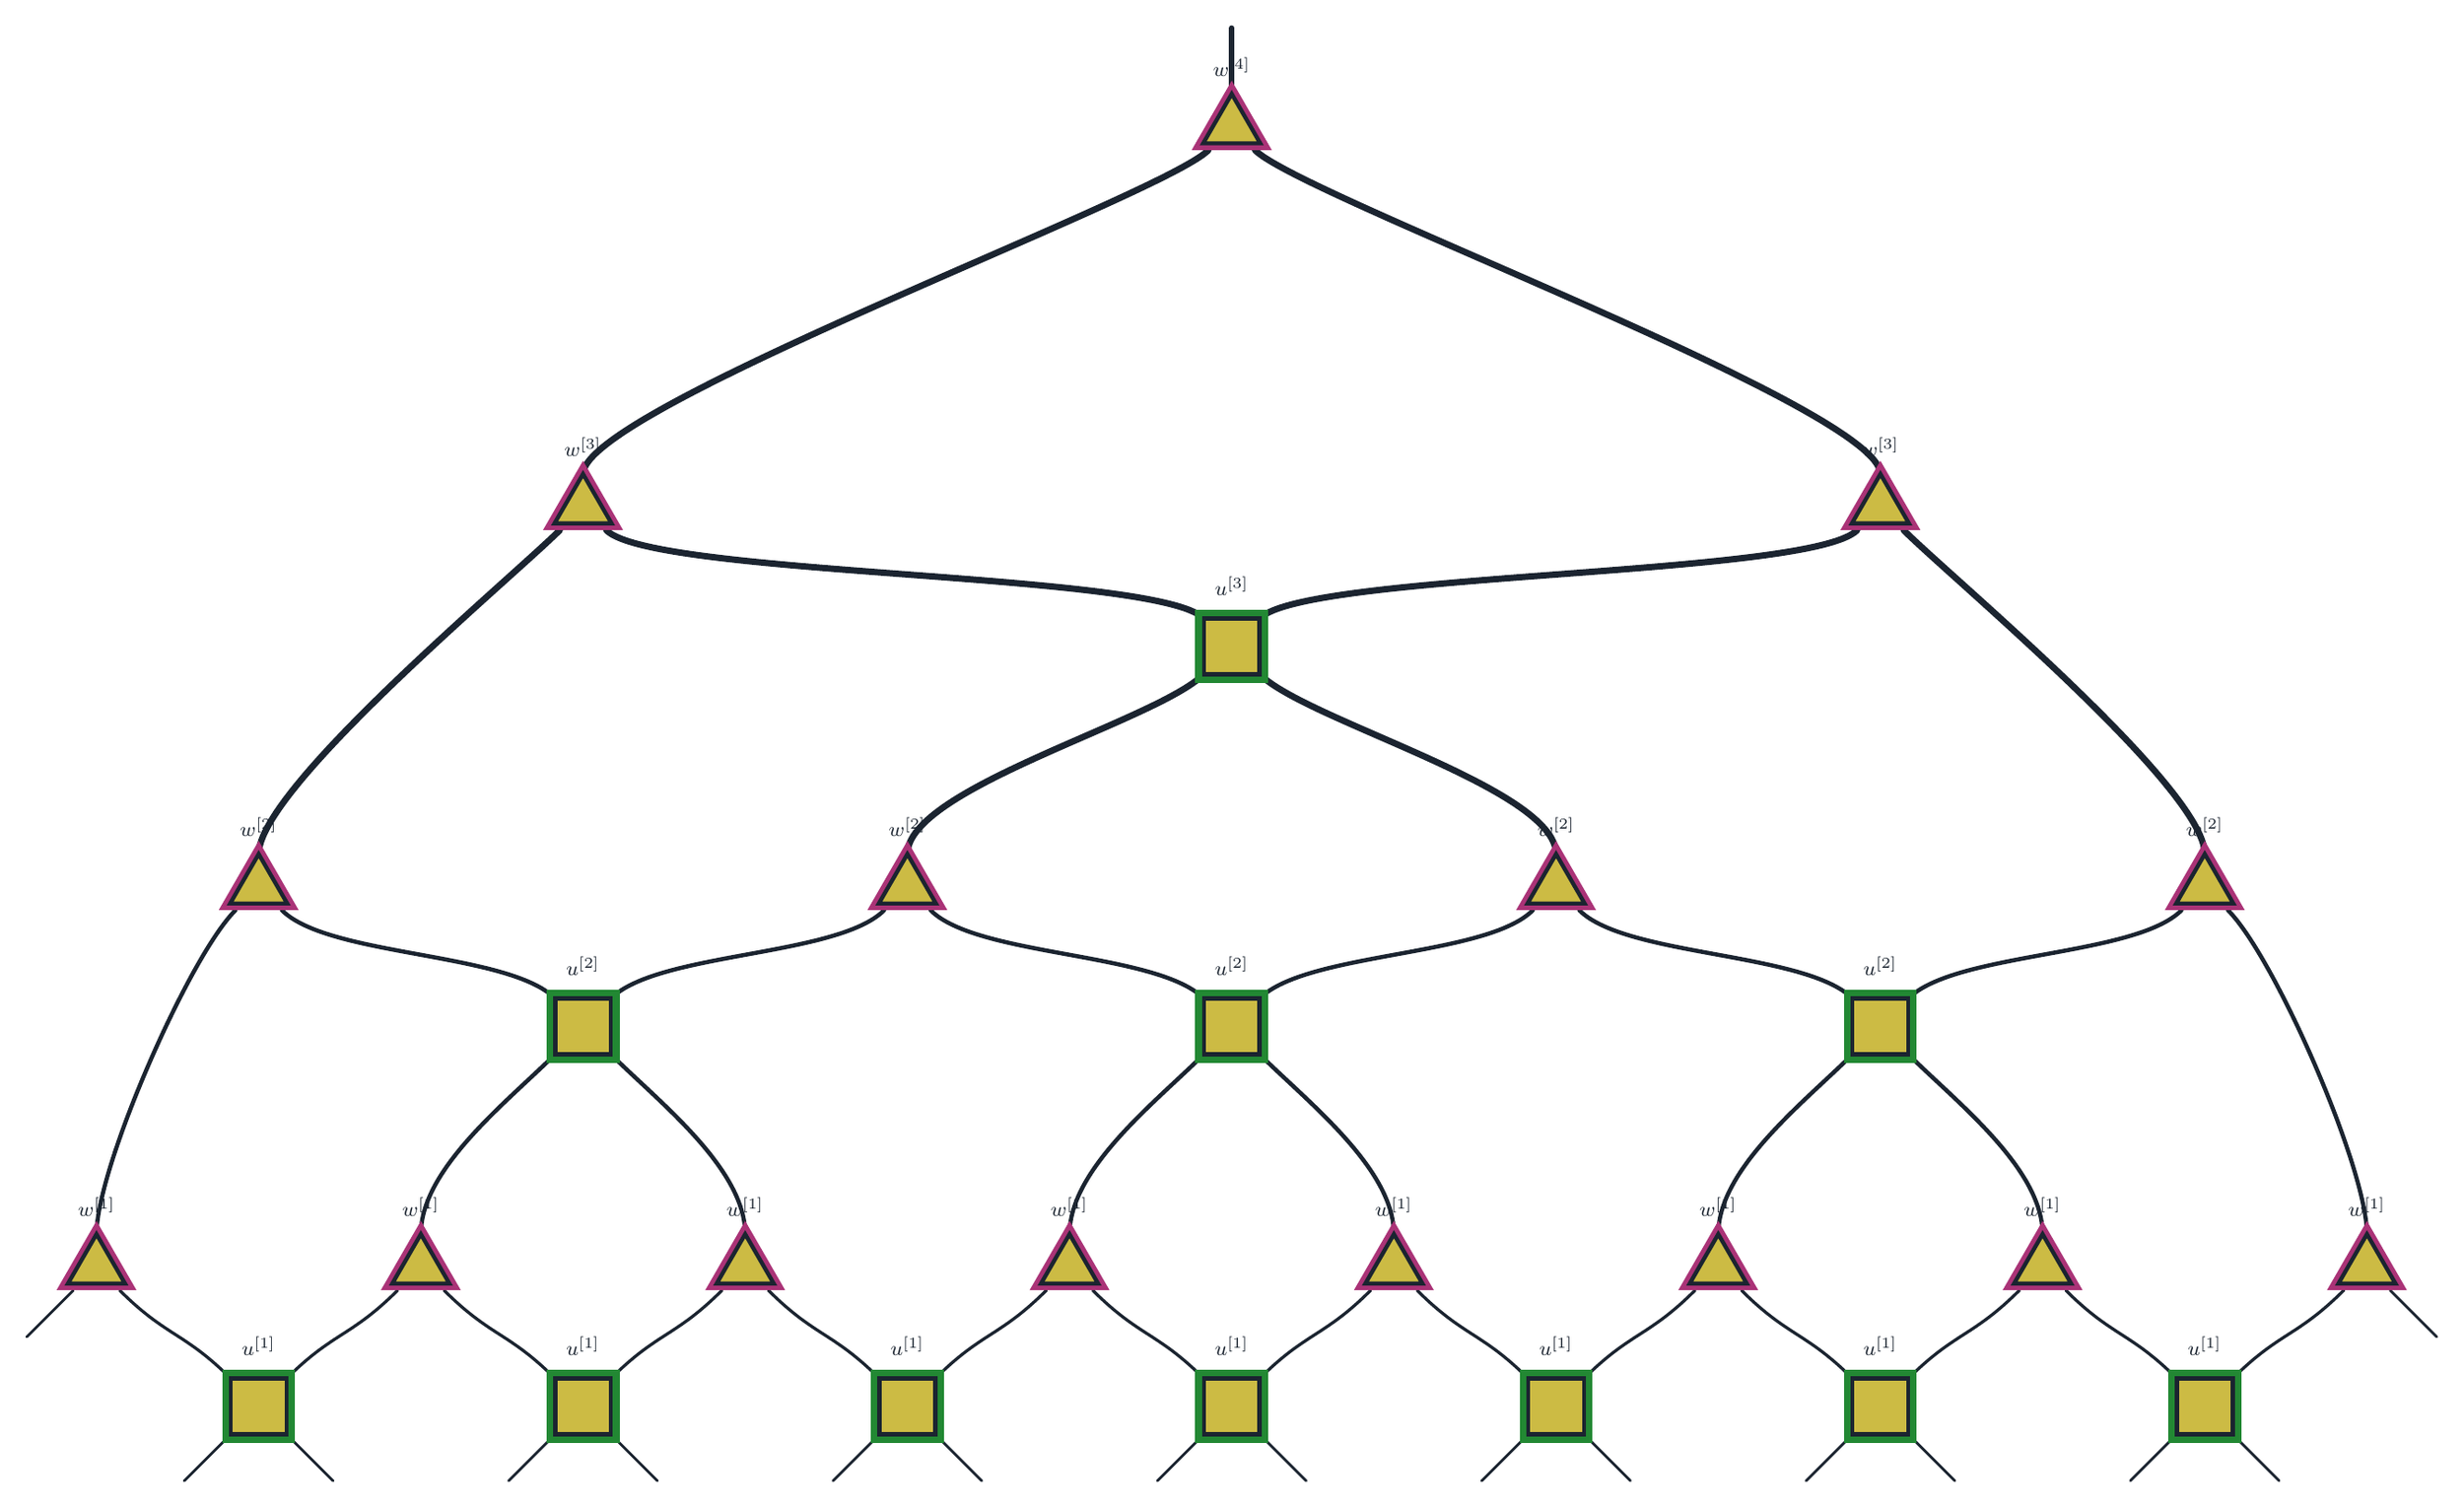
\begin{tikzpicture}[
    x=1pt, y=-1pt,
    moira bond/.style={draw=moiraInk, line cap=round},
    moira leg/.style={draw=moiraInk, line cap=round},
    moira shape/.style={draw=moiraInk, line width=1.6pt},
    moira ring/.style={line width=3pt},
    moira name/.style={text=moiraInk, font=\footnotesize, inner sep=1pt},
]

  % Posições dos tensores.
  \coordinate (t-t13) at (-384,252.5);
  \coordinate (t-t14) at (-256,252.5);
  \coordinate (t-t15) at (-128,252.5);
  \coordinate (t-t16) at (0,252.5);
  \coordinate (t-t17) at (128,252.5);
  \coordinate (t-t18) at (256,252.5);
  \coordinate (t-t19) at (384,252.5);
  \coordinate (t-t20) at (-448,197.5);
  \coordinate (t-t21) at (-320,197.5);
  \coordinate (t-t22) at (-192,197.5);
  \coordinate (t-t23) at (-64,197.5);
  \coordinate (t-t24) at (64,197.5);
  \coordinate (t-t25) at (192,197.5);
  \coordinate (t-t26) at (320,197.5);
  \coordinate (t-t27) at (448,197.5);
  \coordinate (t-t28) at (-256,102.5);
  \coordinate (t-t29) at (0,102.5);
  \coordinate (t-t30) at (256,102.5);
  \coordinate (t-t31) at (-384,47.5);
  \coordinate (t-t32) at (-128,47.5);
  \coordinate (t-t33) at (128,47.5);
  \coordinate (t-t34) at (384,47.5);
  \coordinate (t-t35) at (0,-47.5);
  \coordinate (t-t36) at (-256,-102.5);
  \coordinate (t-t37) at (256,-102.5);
  \coordinate (t-t38) at (0,-252.5);

  % Vínculos.
  \draw[moira bond, line width=1.2pt] ($(t-t13)+(-11,-11)$) .. controls ($(t-t13)+(-29.38,-29.38)$) and ($(t-t20)+(27.58,27.58)$) .. ($(t-t20)+(9.19,9.19)$);
  \draw[moira bond, line width=1.2pt] ($(t-t13)+(11,-11)$) .. controls ($(t-t13)+(29.38,-29.38)$) and ($(t-t21)+(-27.58,27.58)$) .. ($(t-t21)+(-9.19,9.19)$);
  \draw[moira bond, line width=1.2pt] ($(t-t14)+(-11,-11)$) .. controls ($(t-t14)+(-29.38,-29.38)$) and ($(t-t21)+(27.58,27.58)$) .. ($(t-t21)+(9.19,9.19)$);
  \draw[moira bond, line width=1.2pt] ($(t-t14)+(11,-11)$) .. controls ($(t-t14)+(29.38,-29.38)$) and ($(t-t22)+(-27.58,27.58)$) .. ($(t-t22)+(-9.19,9.19)$);
  \draw[moira bond, line width=1.2pt] ($(t-t15)+(-11,-11)$) .. controls ($(t-t15)+(-29.38,-29.38)$) and ($(t-t22)+(27.58,27.58)$) .. ($(t-t22)+(9.19,9.19)$);
  \draw[moira bond, line width=1.2pt] ($(t-t15)+(11,-11)$) .. controls ($(t-t15)+(29.38,-29.38)$) and ($(t-t23)+(-27.58,27.58)$) .. ($(t-t23)+(-9.19,9.19)$);
  \draw[moira bond, line width=1.2pt] ($(t-t16)+(-11,-11)$) .. controls ($(t-t16)+(-29.38,-29.38)$) and ($(t-t23)+(27.58,27.58)$) .. ($(t-t23)+(9.19,9.19)$);
  \draw[moira bond, line width=1.2pt] ($(t-t16)+(11,-11)$) .. controls ($(t-t16)+(29.38,-29.38)$) and ($(t-t24)+(-27.58,27.58)$) .. ($(t-t24)+(-9.19,9.19)$);
  \draw[moira bond, line width=1.2pt] ($(t-t17)+(-11,-11)$) .. controls ($(t-t17)+(-29.38,-29.38)$) and ($(t-t24)+(27.58,27.58)$) .. ($(t-t24)+(9.19,9.19)$);
  \draw[moira bond, line width=1.2pt] ($(t-t17)+(11,-11)$) .. controls ($(t-t17)+(29.38,-29.38)$) and ($(t-t25)+(-27.58,27.58)$) .. ($(t-t25)+(-9.19,9.19)$);
  \draw[moira bond, line width=1.2pt] ($(t-t18)+(-11,-11)$) .. controls ($(t-t18)+(-29.38,-29.38)$) and ($(t-t25)+(27.58,27.58)$) .. ($(t-t25)+(9.19,9.19)$);
  \draw[moira bond, line width=1.2pt] ($(t-t18)+(11,-11)$) .. controls ($(t-t18)+(29.38,-29.38)$) and ($(t-t26)+(-27.58,27.58)$) .. ($(t-t26)+(-9.19,9.19)$);
  \draw[moira bond, line width=1.2pt] ($(t-t19)+(-11,-11)$) .. controls ($(t-t19)+(-29.38,-29.38)$) and ($(t-t26)+(27.58,27.58)$) .. ($(t-t26)+(9.19,9.19)$);
  \draw[moira bond, line width=1.2pt] ($(t-t19)+(11,-11)$) .. controls ($(t-t19)+(29.38,-29.38)$) and ($(t-t27)+(-27.58,27.58)$) .. ($(t-t27)+(-9.19,9.19)$);
  \draw[moira bond, line width=1.64pt] ($(t-t21)+(0,-13)$) .. controls ($(t-t21)+(0,-39)$) and ($(t-t28)+(-29.38,29.38)$) .. ($(t-t28)+(-11,11)$);
  \draw[moira bond, line width=1.64pt] ($(t-t22)+(0,-13)$) .. controls ($(t-t22)+(0,-39)$) and ($(t-t28)+(29.38,29.38)$) .. ($(t-t28)+(11,11)$);
  \draw[moira bond, line width=1.64pt] ($(t-t23)+(0,-13)$) .. controls ($(t-t23)+(0,-39)$) and ($(t-t29)+(-29.38,29.38)$) .. ($(t-t29)+(-11,11)$);
  \draw[moira bond, line width=1.64pt] ($(t-t24)+(0,-13)$) .. controls ($(t-t24)+(0,-39)$) and ($(t-t29)+(29.38,29.38)$) .. ($(t-t29)+(11,11)$);
  \draw[moira bond, line width=1.64pt] ($(t-t25)+(0,-13)$) .. controls ($(t-t25)+(0,-39)$) and ($(t-t30)+(-29.38,29.38)$) .. ($(t-t30)+(-11,11)$);
  \draw[moira bond, line width=1.64pt] ($(t-t26)+(0,-13)$) .. controls ($(t-t26)+(0,-39)$) and ($(t-t30)+(29.38,29.38)$) .. ($(t-t30)+(11,11)$);
  \draw[moira bond, line width=1.64pt] ($(t-t20)+(0,-13)$) .. controls ($(t-t20)+(0,-39)$) and ($(t-t31)+(-27.58,27.58)$) .. ($(t-t31)+(-9.19,9.19)$);
  \draw[moira bond, line width=1.64pt] ($(t-t28)+(-11,-11)$) .. controls ($(t-t28)+(-29.38,-29.38)$) and ($(t-t31)+(27.58,27.58)$) .. ($(t-t31)+(9.19,9.19)$);
  \draw[moira bond, line width=1.64pt] ($(t-t28)+(11,-11)$) .. controls ($(t-t28)+(29.38,-29.38)$) and ($(t-t32)+(-27.58,27.58)$) .. ($(t-t32)+(-9.19,9.19)$);
  \draw[moira bond, line width=1.64pt] ($(t-t29)+(-11,-11)$) .. controls ($(t-t29)+(-29.38,-29.38)$) and ($(t-t32)+(27.58,27.58)$) .. ($(t-t32)+(9.19,9.19)$);
  \draw[moira bond, line width=1.64pt] ($(t-t29)+(11,-11)$) .. controls ($(t-t29)+(29.38,-29.38)$) and ($(t-t33)+(-27.58,27.58)$) .. ($(t-t33)+(-9.19,9.19)$);
  \draw[moira bond, line width=1.64pt] ($(t-t30)+(-11,-11)$) .. controls ($(t-t30)+(-29.38,-29.38)$) and ($(t-t33)+(27.58,27.58)$) .. ($(t-t33)+(9.19,9.19)$);
  \draw[moira bond, line width=1.64pt] ($(t-t30)+(11,-11)$) .. controls ($(t-t30)+(29.38,-29.38)$) and ($(t-t34)+(-27.58,27.58)$) .. ($(t-t34)+(-9.19,9.19)$);
  \draw[moira bond, line width=1.64pt] ($(t-t27)+(0,-13)$) .. controls ($(t-t27)+(0,-39)$) and ($(t-t34)+(27.58,27.58)$) .. ($(t-t34)+(9.19,9.19)$);
  \draw[moira bond, line width=2.51pt] ($(t-t32)+(0,-13)$) .. controls ($(t-t32)+(0,-39)$) and ($(t-t35)+(-29.38,29.38)$) .. ($(t-t35)+(-11,11)$);
  \draw[moira bond, line width=2.51pt] ($(t-t33)+(0,-13)$) .. controls ($(t-t33)+(0,-39)$) and ($(t-t35)+(29.38,29.38)$) .. ($(t-t35)+(11,11)$);
  \draw[moira bond, line width=2.51pt] ($(t-t31)+(0,-13)$) .. controls ($(t-t31)+(0,-39)$) and ($(t-t36)+(-27.58,27.58)$) .. ($(t-t36)+(-9.19,9.19)$);
  \draw[moira bond, line width=2.51pt] ($(t-t35)+(-11,-11)$) .. controls ($(t-t35)+(-29.38,-29.38)$) and ($(t-t36)+(27.58,27.58)$) .. ($(t-t36)+(9.19,9.19)$);
  \draw[moira bond, line width=2.51pt] ($(t-t35)+(11,-11)$) .. controls ($(t-t35)+(29.38,-29.38)$) and ($(t-t37)+(-27.58,27.58)$) .. ($(t-t37)+(-9.19,9.19)$);
  \draw[moira bond, line width=2.51pt] ($(t-t34)+(0,-13)$) .. controls ($(t-t34)+(0,-39)$) and ($(t-t37)+(27.58,27.58)$) .. ($(t-t37)+(9.19,9.19)$);
  \draw[moira bond, line width=2.51pt] ($(t-t36)+(0,-13)$) .. controls ($(t-t36)+(0,-39)$) and ($(t-t38)+(-27.58,27.58)$) .. ($(t-t38)+(-9.19,9.19)$);
  \draw[moira bond, line width=2.51pt] ($(t-t37)+(0,-13)$) .. controls ($(t-t37)+(0,-39)$) and ($(t-t38)+(27.58,27.58)$) .. ($(t-t38)+(9.19,9.19)$);

  % Pernas livres.
  \draw[moira leg, line width=1.02pt] ($(t-t13)+(-11,11)$) -- ($(t-t13)+(-29.38,29.38)$);
  \draw[moira leg, line width=1.02pt] ($(t-t13)+(11,11)$) -- ($(t-t13)+(29.38,29.38)$);
  \draw[moira leg, line width=1.02pt] ($(t-t14)+(-11,11)$) -- ($(t-t14)+(-29.38,29.38)$);
  \draw[moira leg, line width=1.02pt] ($(t-t14)+(11,11)$) -- ($(t-t14)+(29.38,29.38)$);
  \draw[moira leg, line width=1.02pt] ($(t-t15)+(-11,11)$) -- ($(t-t15)+(-29.38,29.38)$);
  \draw[moira leg, line width=1.02pt] ($(t-t15)+(11,11)$) -- ($(t-t15)+(29.38,29.38)$);
  \draw[moira leg, line width=1.02pt] ($(t-t16)+(-11,11)$) -- ($(t-t16)+(-29.38,29.38)$);
  \draw[moira leg, line width=1.02pt] ($(t-t16)+(11,11)$) -- ($(t-t16)+(29.38,29.38)$);
  \draw[moira leg, line width=1.02pt] ($(t-t17)+(-11,11)$) -- ($(t-t17)+(-29.38,29.38)$);
  \draw[moira leg, line width=1.02pt] ($(t-t17)+(11,11)$) -- ($(t-t17)+(29.38,29.38)$);
  \draw[moira leg, line width=1.02pt] ($(t-t18)+(-11,11)$) -- ($(t-t18)+(-29.38,29.38)$);
  \draw[moira leg, line width=1.02pt] ($(t-t18)+(11,11)$) -- ($(t-t18)+(29.38,29.38)$);
  \draw[moira leg, line width=1.02pt] ($(t-t19)+(-11,11)$) -- ($(t-t19)+(-29.38,29.38)$);
  \draw[moira leg, line width=1.02pt] ($(t-t19)+(11,11)$) -- ($(t-t19)+(29.38,29.38)$);
  \draw[moira leg, line width=1.02pt] ($(t-t20)+(-9.19,9.19)$) -- ($(t-t20)+(-27.58,27.58)$);
  \draw[moira leg, line width=1.02pt] ($(t-t27)+(9.19,9.19)$) -- ($(t-t27)+(27.58,27.58)$);
  \draw[moira leg, line width=2.13pt] ($(t-t38)+(0,-13)$) -- ($(t-t38)+(0,-39)$);

  % Tensores.
  \draw[moira ring, draw=moiraGreen] ($(t-t13)+(-12.87,-12.87)$) -- ($(t-t13)+(12.87,-12.87)$) -- ($(t-t13)+(12.87,12.87)$) -- ($(t-t13)+(-12.87,12.87)$) -- cycle;
  \draw[moira shape, fill=moiraAmber] ($(t-t13)+(-11,-11)$) -- ($(t-t13)+(11,-11)$) -- ($(t-t13)+(11,11)$) -- ($(t-t13)+(-11,11)$) -- cycle;
  \draw[moira ring, draw=moiraGreen] ($(t-t14)+(-12.87,-12.87)$) -- ($(t-t14)+(12.87,-12.87)$) -- ($(t-t14)+(12.87,12.87)$) -- ($(t-t14)+(-12.87,12.87)$) -- cycle;
  \draw[moira shape, fill=moiraAmber] ($(t-t14)+(-11,-11)$) -- ($(t-t14)+(11,-11)$) -- ($(t-t14)+(11,11)$) -- ($(t-t14)+(-11,11)$) -- cycle;
  \draw[moira ring, draw=moiraGreen] ($(t-t15)+(-12.87,-12.87)$) -- ($(t-t15)+(12.87,-12.87)$) -- ($(t-t15)+(12.87,12.87)$) -- ($(t-t15)+(-12.87,12.87)$) -- cycle;
  \draw[moira shape, fill=moiraAmber] ($(t-t15)+(-11,-11)$) -- ($(t-t15)+(11,-11)$) -- ($(t-t15)+(11,11)$) -- ($(t-t15)+(-11,11)$) -- cycle;
  \draw[moira ring, draw=moiraGreen] ($(t-t16)+(-12.87,-12.87)$) -- ($(t-t16)+(12.87,-12.87)$) -- ($(t-t16)+(12.87,12.87)$) -- ($(t-t16)+(-12.87,12.87)$) -- cycle;
  \draw[moira shape, fill=moiraAmber] ($(t-t16)+(-11,-11)$) -- ($(t-t16)+(11,-11)$) -- ($(t-t16)+(11,11)$) -- ($(t-t16)+(-11,11)$) -- cycle;
  \draw[moira ring, draw=moiraGreen] ($(t-t17)+(-12.87,-12.87)$) -- ($(t-t17)+(12.87,-12.87)$) -- ($(t-t17)+(12.87,12.87)$) -- ($(t-t17)+(-12.87,12.87)$) -- cycle;
  \draw[moira shape, fill=moiraAmber] ($(t-t17)+(-11,-11)$) -- ($(t-t17)+(11,-11)$) -- ($(t-t17)+(11,11)$) -- ($(t-t17)+(-11,11)$) -- cycle;
  \draw[moira ring, draw=moiraGreen] ($(t-t18)+(-12.87,-12.87)$) -- ($(t-t18)+(12.87,-12.87)$) -- ($(t-t18)+(12.87,12.87)$) -- ($(t-t18)+(-12.87,12.87)$) -- cycle;
  \draw[moira shape, fill=moiraAmber] ($(t-t18)+(-11,-11)$) -- ($(t-t18)+(11,-11)$) -- ($(t-t18)+(11,11)$) -- ($(t-t18)+(-11,11)$) -- cycle;
  \draw[moira ring, draw=moiraGreen] ($(t-t19)+(-12.87,-12.87)$) -- ($(t-t19)+(12.87,-12.87)$) -- ($(t-t19)+(12.87,12.87)$) -- ($(t-t19)+(-12.87,12.87)$) -- cycle;
  \draw[moira shape, fill=moiraAmber] ($(t-t19)+(-11,-11)$) -- ($(t-t19)+(11,-11)$) -- ($(t-t19)+(11,11)$) -- ($(t-t19)+(-11,11)$) -- cycle;
  \draw[moira ring, draw=moiraPurple] ($(t-t20)+(0,-15.21)$) -- ($(t-t20)+(13.17,7.61)$) -- ($(t-t20)+(-13.17,7.61)$) -- cycle;
  \draw[moira shape, fill=moiraAmber] ($(t-t20)+(0,-13)$) -- ($(t-t20)+(11.26,6.5)$) -- ($(t-t20)+(-11.26,6.5)$) -- cycle;
  \draw[moira ring, draw=moiraPurple] ($(t-t21)+(0,-15.21)$) -- ($(t-t21)+(13.17,7.61)$) -- ($(t-t21)+(-13.17,7.61)$) -- cycle;
  \draw[moira shape, fill=moiraAmber] ($(t-t21)+(0,-13)$) -- ($(t-t21)+(11.26,6.5)$) -- ($(t-t21)+(-11.26,6.5)$) -- cycle;
  \draw[moira ring, draw=moiraPurple] ($(t-t22)+(0,-15.21)$) -- ($(t-t22)+(13.17,7.61)$) -- ($(t-t22)+(-13.17,7.61)$) -- cycle;
  \draw[moira shape, fill=moiraAmber] ($(t-t22)+(0,-13)$) -- ($(t-t22)+(11.26,6.5)$) -- ($(t-t22)+(-11.26,6.5)$) -- cycle;
  \draw[moira ring, draw=moiraPurple] ($(t-t23)+(0,-15.21)$) -- ($(t-t23)+(13.17,7.61)$) -- ($(t-t23)+(-13.17,7.61)$) -- cycle;
  \draw[moira shape, fill=moiraAmber] ($(t-t23)+(0,-13)$) -- ($(t-t23)+(11.26,6.5)$) -- ($(t-t23)+(-11.26,6.5)$) -- cycle;
  \draw[moira ring, draw=moiraPurple] ($(t-t24)+(0,-15.21)$) -- ($(t-t24)+(13.17,7.61)$) -- ($(t-t24)+(-13.17,7.61)$) -- cycle;
  \draw[moira shape, fill=moiraAmber] ($(t-t24)+(0,-13)$) -- ($(t-t24)+(11.26,6.5)$) -- ($(t-t24)+(-11.26,6.5)$) -- cycle;
  \draw[moira ring, draw=moiraPurple] ($(t-t25)+(0,-15.21)$) -- ($(t-t25)+(13.17,7.61)$) -- ($(t-t25)+(-13.17,7.61)$) -- cycle;
  \draw[moira shape, fill=moiraAmber] ($(t-t25)+(0,-13)$) -- ($(t-t25)+(11.26,6.5)$) -- ($(t-t25)+(-11.26,6.5)$) -- cycle;
  \draw[moira ring, draw=moiraPurple] ($(t-t26)+(0,-15.21)$) -- ($(t-t26)+(13.17,7.61)$) -- ($(t-t26)+(-13.17,7.61)$) -- cycle;
  \draw[moira shape, fill=moiraAmber] ($(t-t26)+(0,-13)$) -- ($(t-t26)+(11.26,6.5)$) -- ($(t-t26)+(-11.26,6.5)$) -- cycle;
  \draw[moira ring, draw=moiraPurple] ($(t-t27)+(0,-15.21)$) -- ($(t-t27)+(13.17,7.61)$) -- ($(t-t27)+(-13.17,7.61)$) -- cycle;
  \draw[moira shape, fill=moiraAmber] ($(t-t27)+(0,-13)$) -- ($(t-t27)+(11.26,6.5)$) -- ($(t-t27)+(-11.26,6.5)$) -- cycle;
  \draw[moira ring, draw=moiraGreen] ($(t-t28)+(-12.87,-12.87)$) -- ($(t-t28)+(12.87,-12.87)$) -- ($(t-t28)+(12.87,12.87)$) -- ($(t-t28)+(-12.87,12.87)$) -- cycle;
  \draw[moira shape, fill=moiraAmber] ($(t-t28)+(-11,-11)$) -- ($(t-t28)+(11,-11)$) -- ($(t-t28)+(11,11)$) -- ($(t-t28)+(-11,11)$) -- cycle;
  \draw[moira ring, draw=moiraGreen] ($(t-t29)+(-12.87,-12.87)$) -- ($(t-t29)+(12.87,-12.87)$) -- ($(t-t29)+(12.87,12.87)$) -- ($(t-t29)+(-12.87,12.87)$) -- cycle;
  \draw[moira shape, fill=moiraAmber] ($(t-t29)+(-11,-11)$) -- ($(t-t29)+(11,-11)$) -- ($(t-t29)+(11,11)$) -- ($(t-t29)+(-11,11)$) -- cycle;
  \draw[moira ring, draw=moiraGreen] ($(t-t30)+(-12.87,-12.87)$) -- ($(t-t30)+(12.87,-12.87)$) -- ($(t-t30)+(12.87,12.87)$) -- ($(t-t30)+(-12.87,12.87)$) -- cycle;
  \draw[moira shape, fill=moiraAmber] ($(t-t30)+(-11,-11)$) -- ($(t-t30)+(11,-11)$) -- ($(t-t30)+(11,11)$) -- ($(t-t30)+(-11,11)$) -- cycle;
  \draw[moira ring, draw=moiraPurple] ($(t-t31)+(0,-15.21)$) -- ($(t-t31)+(13.17,7.61)$) -- ($(t-t31)+(-13.17,7.61)$) -- cycle;
  \draw[moira shape, fill=moiraAmber] ($(t-t31)+(0,-13)$) -- ($(t-t31)+(11.26,6.5)$) -- ($(t-t31)+(-11.26,6.5)$) -- cycle;
  \draw[moira ring, draw=moiraPurple] ($(t-t32)+(0,-15.21)$) -- ($(t-t32)+(13.17,7.61)$) -- ($(t-t32)+(-13.17,7.61)$) -- cycle;
  \draw[moira shape, fill=moiraAmber] ($(t-t32)+(0,-13)$) -- ($(t-t32)+(11.26,6.5)$) -- ($(t-t32)+(-11.26,6.5)$) -- cycle;
  \draw[moira ring, draw=moiraPurple] ($(t-t33)+(0,-15.21)$) -- ($(t-t33)+(13.17,7.61)$) -- ($(t-t33)+(-13.17,7.61)$) -- cycle;
  \draw[moira shape, fill=moiraAmber] ($(t-t33)+(0,-13)$) -- ($(t-t33)+(11.26,6.5)$) -- ($(t-t33)+(-11.26,6.5)$) -- cycle;
  \draw[moira ring, draw=moiraPurple] ($(t-t34)+(0,-15.21)$) -- ($(t-t34)+(13.17,7.61)$) -- ($(t-t34)+(-13.17,7.61)$) -- cycle;
  \draw[moira shape, fill=moiraAmber] ($(t-t34)+(0,-13)$) -- ($(t-t34)+(11.26,6.5)$) -- ($(t-t34)+(-11.26,6.5)$) -- cycle;
  \draw[moira ring, draw=moiraGreen] ($(t-t35)+(-12.87,-12.87)$) -- ($(t-t35)+(12.87,-12.87)$) -- ($(t-t35)+(12.87,12.87)$) -- ($(t-t35)+(-12.87,12.87)$) -- cycle;
  \draw[moira shape, fill=moiraAmber] ($(t-t35)+(-11,-11)$) -- ($(t-t35)+(11,-11)$) -- ($(t-t35)+(11,11)$) -- ($(t-t35)+(-11,11)$) -- cycle;
  \draw[moira ring, draw=moiraPurple] ($(t-t36)+(0,-15.21)$) -- ($(t-t36)+(13.17,7.61)$) -- ($(t-t36)+(-13.17,7.61)$) -- cycle;
  \draw[moira shape, fill=moiraAmber] ($(t-t36)+(0,-13)$) -- ($(t-t36)+(11.26,6.5)$) -- ($(t-t36)+(-11.26,6.5)$) -- cycle;
  \draw[moira ring, draw=moiraPurple] ($(t-t37)+(0,-15.21)$) -- ($(t-t37)+(13.17,7.61)$) -- ($(t-t37)+(-13.17,7.61)$) -- cycle;
  \draw[moira shape, fill=moiraAmber] ($(t-t37)+(0,-13)$) -- ($(t-t37)+(11.26,6.5)$) -- ($(t-t37)+(-11.26,6.5)$) -- cycle;
  \draw[moira ring, draw=moiraPurple] ($(t-t38)+(0,-15.21)$) -- ($(t-t38)+(13.17,7.61)$) -- ($(t-t38)+(-13.17,7.61)$) -- cycle;
  \draw[moira shape, fill=moiraAmber] ($(t-t38)+(0,-13)$) -- ($(t-t38)+(11.26,6.5)$) -- ($(t-t38)+(-11.26,6.5)$) -- cycle;

  % Rótulos.
  \node[moira name, anchor=base] at ($(t-t13)+(0,-20)$) {$u^{[1]}$};
  \node[moira name, anchor=base] at ($(t-t14)+(0,-20)$) {$u^{[1]}$};
  \node[moira name, anchor=base] at ($(t-t15)+(0,-20)$) {$u^{[1]}$};
  \node[moira name, anchor=base] at ($(t-t16)+(0,-20)$) {$u^{[1]}$};
  \node[moira name, anchor=base] at ($(t-t17)+(0,-20)$) {$u^{[1]}$};
  \node[moira name, anchor=base] at ($(t-t18)+(0,-20)$) {$u^{[1]}$};
  \node[moira name, anchor=base] at ($(t-t19)+(0,-20)$) {$u^{[1]}$};
  \node[moira name, anchor=base] at ($(t-t20)+(0,-20)$) {$w^{[1]}$};
  \node[moira name, anchor=base] at ($(t-t21)+(0,-20)$) {$w^{[1]}$};
  \node[moira name, anchor=base] at ($(t-t22)+(0,-20)$) {$w^{[1]}$};
  \node[moira name, anchor=base] at ($(t-t23)+(0,-20)$) {$w^{[1]}$};
  \node[moira name, anchor=base] at ($(t-t24)+(0,-20)$) {$w^{[1]}$};
  \node[moira name, anchor=base] at ($(t-t25)+(0,-20)$) {$w^{[1]}$};
  \node[moira name, anchor=base] at ($(t-t26)+(0,-20)$) {$w^{[1]}$};
  \node[moira name, anchor=base] at ($(t-t27)+(0,-20)$) {$w^{[1]}$};
  \node[moira name, anchor=base] at ($(t-t28)+(0,-20)$) {$u^{[2]}$};
  \node[moira name, anchor=base] at ($(t-t29)+(0,-20)$) {$u^{[2]}$};
  \node[moira name, anchor=base] at ($(t-t30)+(0,-20)$) {$u^{[2]}$};
  \node[moira name, anchor=base] at ($(t-t31)+(0,-20)$) {$w^{[2]}$};
  \node[moira name, anchor=base] at ($(t-t32)+(0,-20)$) {$w^{[2]}$};
  \node[moira name, anchor=base] at ($(t-t33)+(0,-20)$) {$w^{[2]}$};
  \node[moira name, anchor=base] at ($(t-t34)+(0,-20)$) {$w^{[2]}$};
  \node[moira name, anchor=base] at ($(t-t35)+(0,-20)$) {$u^{[3]}$};
  \node[moira name, anchor=base] at ($(t-t36)+(0,-20)$) {$w^{[3]}$};
  \node[moira name, anchor=base] at ($(t-t37)+(0,-20)$) {$w^{[3]}$};
  \node[moira name, anchor=base] at ($(t-t38)+(0,-20)$) {$w^{[4]}$};
\end{tikzpicture}
\end{document}
